\ifx\PREAMBLE\undefined
\documentclass{report}
\usepackage[format = hang, font = bf]{caption}
\usepackage{graphicx}
\usepackage{array}
\usepackage{amsmath}
\usepackage{colortbl}
\usepackage{empheq}
\usepackage{mathtools}
\usepackage{boxedminipage}
\usepackage{listings}
\usepackage{makecell}%diagonal line in table
\usepackage{float}%allowing forceful figure[H]
\usepackage{xcolor}
\usepackage{amsfonts}%allowing \mathbb{R}
\usepackage{amssymb}
\usepackage{bm}
\usepackage{alltt}
\usepackage{amsthm}
\usepackage[super]{nth}
\usepackage{tikz}
\usetikzlibrary{positioning, calc}
\usepackage{multirow}
\usepackage{algorithmicx}
\usepackage[chapter]{algorithm} 
%chapter option ensures that algorithms are numbered within each chapter rather than in the whole article
\usepackage[noend]{algpseudocode} %If end if, end procedure, etc is expected to appear, remove the noend option
\usepackage{xspace}
\usepackage{color}
\usepackage{url}
\def\UrlBreaks{\do\A\do\B\do\C\do\D\do\E\do\F\do\G\do\H\do\I\do\J\do\K\do\L\do\M\do\N\do\O\do\P\do\Q\do\R\do\S\do\T\do\U\do\V\do\W\do\X\do\Y\do\Z\do\[\do\\\do\]\do\^\do\_\do\`\do\a\do\b\do\c\do\d\do\e\do\f\do\g\do\h\do\i\do\j\do\k\do\l\do\m\do\n\do\o\do\p\do\q\do\r\do\s\do\t\do\u\do\v\do\w\do\x\do\y\do\z\do\0\do\1\do\2\do\3\do\4\do\5\do\6\do\7\do\8\do\9\do\.\do\@\do\\\do\/\do\!\do\_\do\|\do\;\do\>\do\]\do\)\do\,\do\?\do\'\do+\do\=\do\#\do\-}
\usepackage[breaklinks = true]{hyperref}
\lstset{language = c++, breaklines = true, tabsize = 2, numbers = left, extendedchars = false, basicstyle = {\ttfamily \footnotesize}, keywordstyle=\color{blue!70}, commentstyle=\color{red!70}, frame=shadowbox, rulesepcolor=\color{red!20!green!20!blue!20}, numberstyle={\color[RGB]{0,192,192}}}
\mathchardef\myhyphen="2D
% switch-case environment definitions
\algblock{switch}{endswitch} 
\algblock{case}{endcase}
%\algrenewtext{endswitch}{\textbf{end switch}} %If end switch is expected to appear, uncomment this line.
\algtext*{endswitch} % Make end switch disappear
\algtext*{endcase}
\allowdisplaybreaks
\DeclareMathOperator*{\argmin}{\arg\!\min}
\DeclareMathOperator*{\argmax}{\arg\!\max}

\begin{document}
\fi
\chapter{Introduction}
\section{Cryptographic Hash Functions}
A hash function is a function satisfying the following conditions:
\begin{itemize}
  \item takes any string as input
  \item produces fixed-sized output (256-bit in this course, used by bitcoin)
  \item is efficiently computable
\end{itemize}
\subsection{Security Properties}
A hash function has to satisfy some security properties to be used for cyrptographic purposes.
\subsubsection{Collision Free}
No one can find two inputs that produce the same hash: $x\neq y$ and $H(x)=H(y)$. 
\begin{itemize}
  \item \textit{No one can find} is different from \textit{There does not exist}. Since the size of the output range ($2^{256}$) is way smaller than that of the input range, there exist a lot of collisions. 
  \item Try $2^{130}$ randomly chosen inputs and there is a 99.8\% chance that a collision can be found, but the process takes too long to matter.
  \item No hash function $H$ has been proved to be collision-free. Some functions are believed to be collision-free because enormous efforts have been made to find their collisions without success.
  \item Application: hash as message digest. $H(x)=H(y)$ convinces us that $x=y$. To recognize a file that we met before, just remember its hash. It is useful because hash is usually much smaller than the original input.
\end{itemize}
\subsubsection{Hiding}
Given $H(x)$, it is infeasible to find $x$.
\begin{itemize}
  \item The set from which the input is selected has to be spread out, otherwise an adversary can find $x$ by trying a few likely inputs and compare them against $H(x)$.
  \item In order to achieve hiding, we can concatenate the input with a prefix from a probability distribution with high min-entropy and calculate $H(r|x)$. High min-entropy means that the distribution is \textit{very spread out}, so that no particular value is chosen with more than negligible probability.
  \item Application: commitment. Commit to a value and reveal it later. \textit{Seal a value in an envelope and open the envelope later}. The following API is provided:
  \begin{itemize}
    \item To seal the message in envelope: $(com, key)\coloneqq commit(msg)$. $com$ is published. 
    \item To open the envelope: $match\coloneqq verify(com, key, msg)$. $key, msg$ are published, and anyone can verify the validity of $com$.
  \end{itemize}
  The security properties guarantee that given $com$, it's infeasible to reveal $msg$; neither is it feasible to find another msg that passes the validity check with respect to $com$. We use $H(key|msg)$ as $commit(msg)$, in which $key$ is a random 256-bit value.
\end{itemize}
\subsubsection{Puzzle Friendly}
For every possible output value $y$, if $k$ is chosen randomly from a probability distribution with high min-entropy, then it's infeasible to find $x$ s.t. $H(k|x)=y$.
\begin{itemize}
  \item It's infeasible for an adversary to find an input that produces a target output.
  \item Application: search puzzle. Given a puzzle id from a high min-entropy distribution and a target set $Y$, try to find a solution $x$ s.t. $H(id|x)\in Y$. Puzzle friendly guarantees that there is no better solution than trying random values.
\end{itemize}
\subsection{SHA-256 Hash Function}
The hash function used by bitcoin is the SHA-256 function.
\begin{center}
  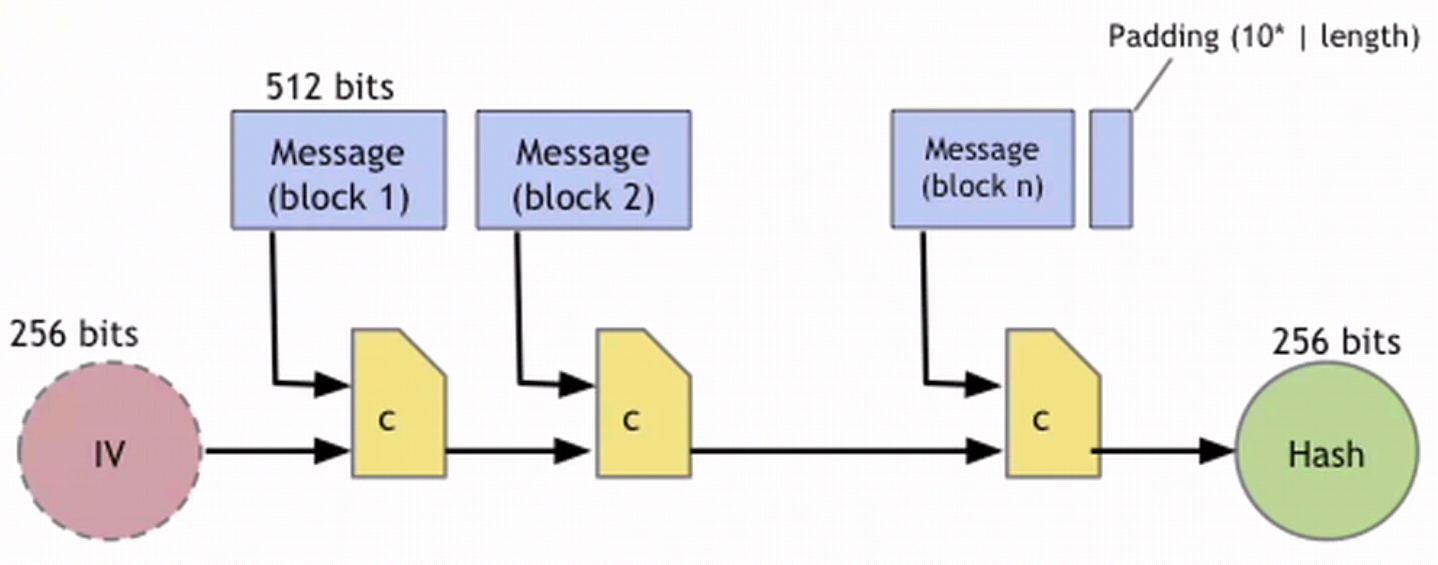
\includegraphics[width=\textwidth]{sha256.png}
\end{center}
\begin{itemize}
  \item Messages are broken into blocks of 512 bits. Padding is added at the end. 10* + 64-bit msg length.
  \item IV is a 256-bit number from the standard.
  \item $c$ is a compression function that outputs 256 bits.
  \item If $c$ is collision-free, then SHA-256 is collision-free.
\end{itemize}
\section{Hash Pointers}
A hash pointer stores the location and cyrptographic hash of some information. With a hash pointer, we can get the information back and very that it hasn't changed. It is often drawn as follows.
\begin{center}
  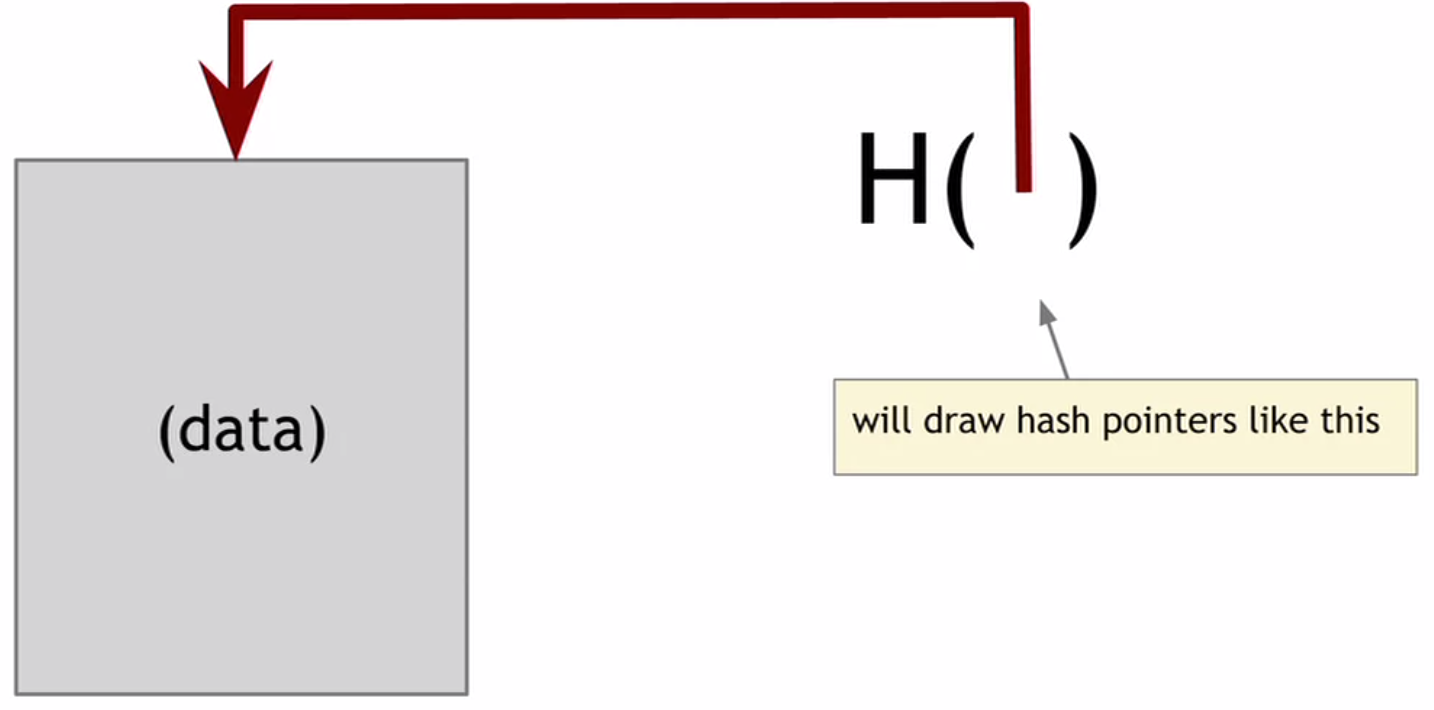
\includegraphics[width=0.7\textwidth]{hashpointer.png}
\end{center}
All acyclic pointer based data structures can be built with hash pointers, in which hash pointers take the role of normal pointers. If there exist cycles, the data structure cannot be built with hash pointers.
\subsection{Linked List}
A linked list built with hash pointers is called a blockchain. The head of the list is remembered, which is sometimes called the Genesis block.
\begin{center}
  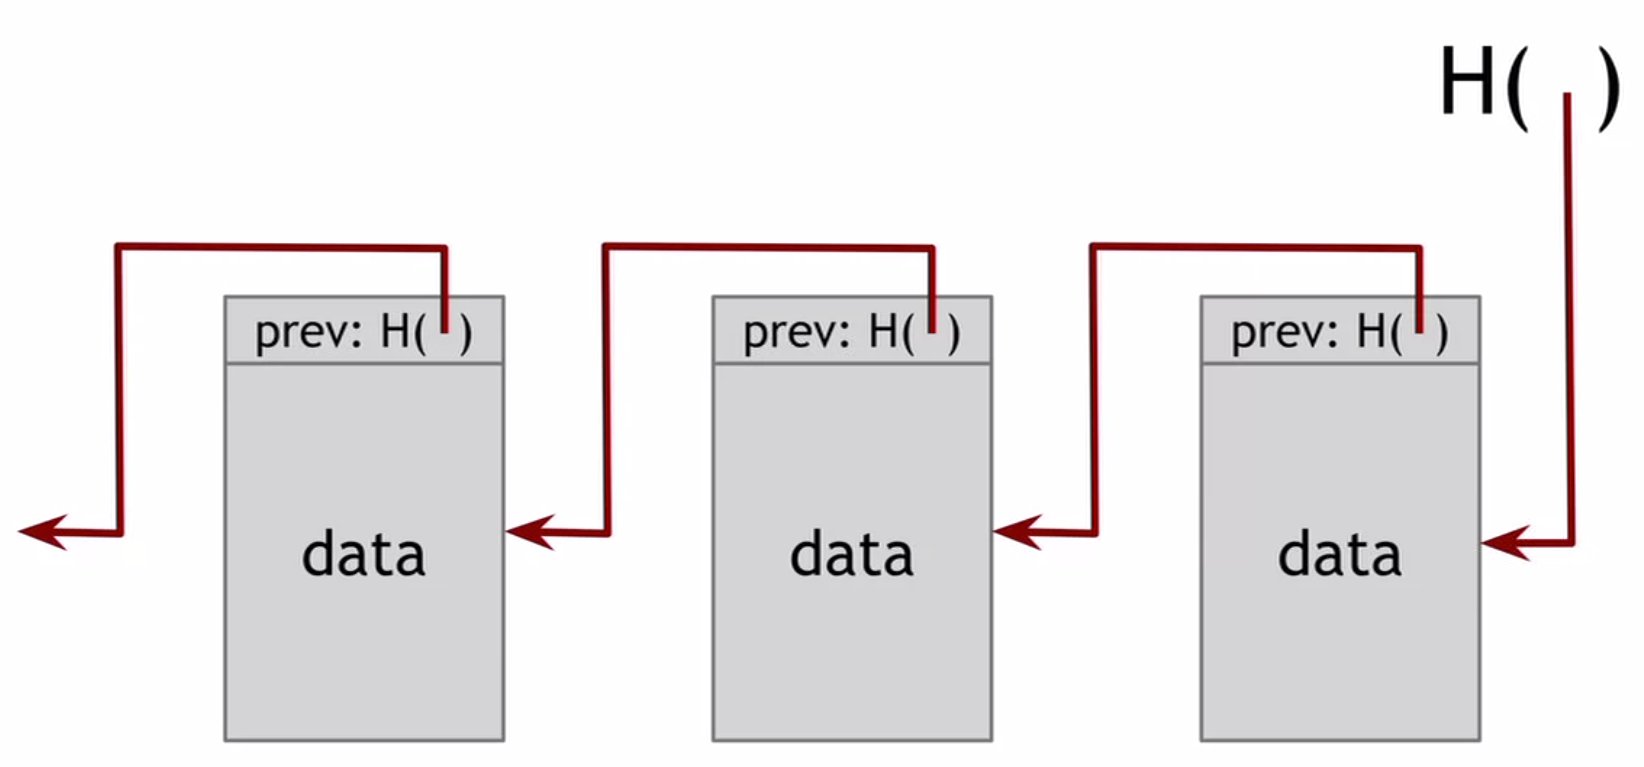
\includegraphics[width=0.7\textwidth]{linklist.png}
\end{center}
Blockchain can be used to build a tamper-evident log. When an adversary wants to modify block $t$ without making the owner of the log realize it, he has to also modify the hash of block $t$ contained in  block $t-1$, which forces him to modify the hash of block $t-1$ contained in block $t-2\dots$ As a result, any attempt to modify a block results in modifying the head of the list, which is impossible because it has been remembered.
\subsection{Binary Tree (Merkle Tree)}
\begin{center}
  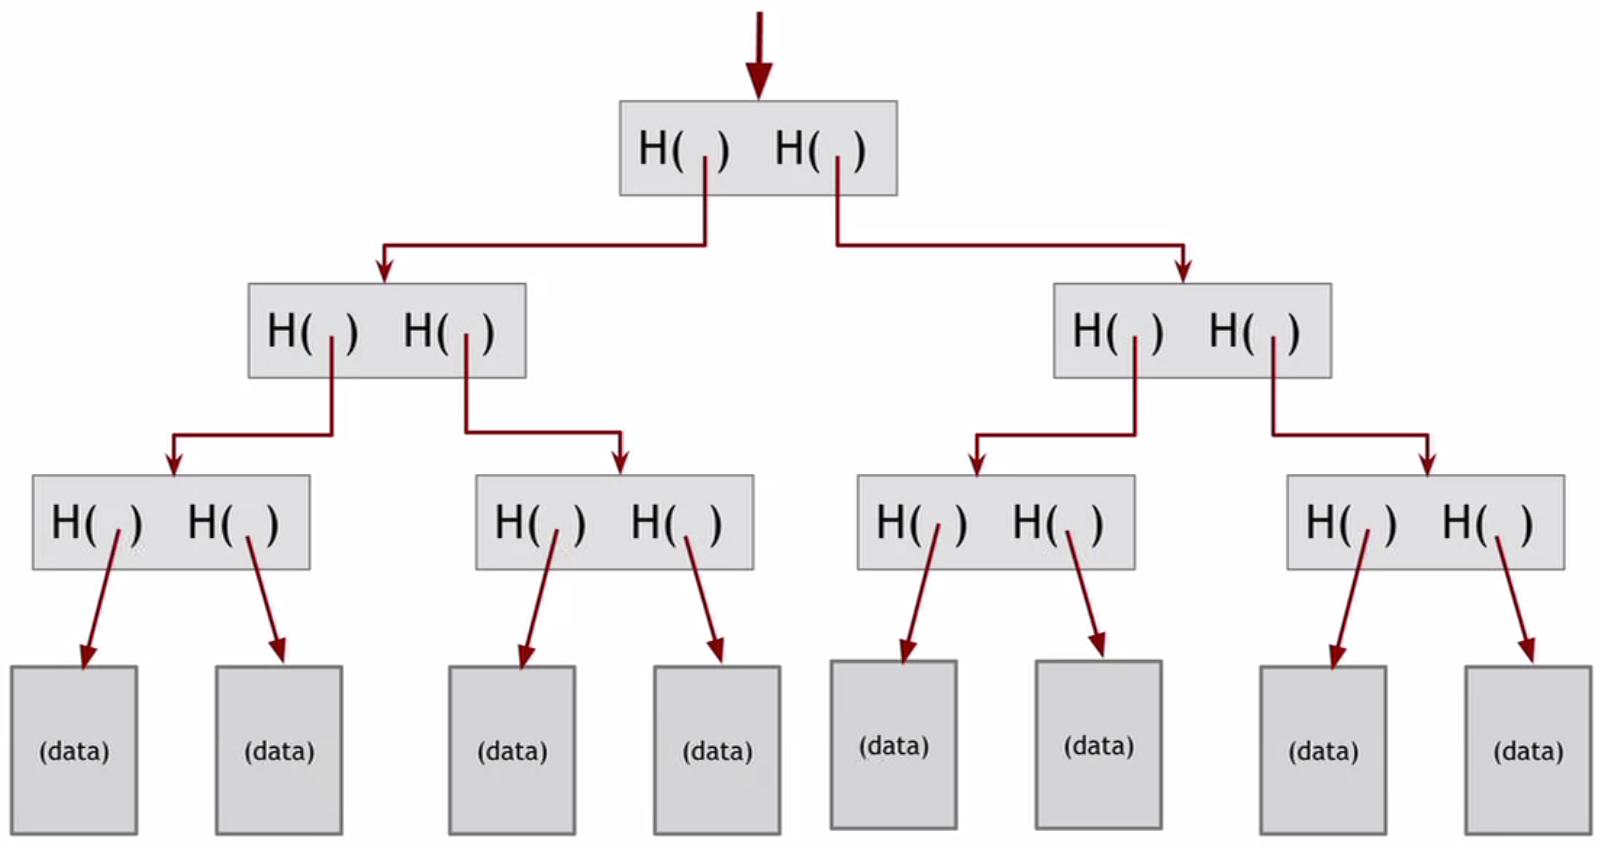
\includegraphics[width=\textwidth]{merkletree.png}
\end{center}
Advantages of Merkle tree: 
\begin{itemize}
  \item The tree holds many items but only the root hash needs to be remembered.
  \item Membership can be verified in $O(\log n)$ time and space: only the blocks along the path to the root is needed. Blockchain needs $O(n)$ time.
  \item A sorted Merkle tree can verify non-membership in $O(\log n)$ by showing the two consecutive blocks that would be before and after the target block if it were in the tree. 
\end{itemize}
\section{Digital Signatures}
Digital Signature is just like a normal signature on paper, only in digital form.
\begin{itemize}
  \item Only you can sign but anyone can verify.
  \item Signature is tied to a particular document. It cannot be cut-and-pasted to another document.
\end{itemize}
\subsection{APIs}
\begin{itemize}
  \item Key generation: $(sk, pk)\coloneqq generateKeys(keySize)$
  \begin{itemize}
    \item $sk$: secret signing key. $pk$: public verification key
  \end{itemize}
  \item Sign operation: $sig\coloneqq sign(sk, message)$
  \item Verification operation: $isValid\coloneqq verify(pk, message, sig)$
\end{itemize}
The first two can be randomized algorithms. The verification algorithm cannot be random. The verification algorithm should satisfy 
\[verify(pk, message, sign(sk, message)) == true \]
\subsection{Digital Signature Chanllenge Game}
It should be guaranteed that an adversary who knows $pk$ and can obtain signatures on messages of his choice cannot forge a verifiable signature on another message. This can be checked with a game:
\begin{itemize}
  \item A pair of keys $(sk, pk)$ is generated. $sk$ is given to the challenger and $pk$ is given to both the challenger and the adversary.
  \item The adversary can name any message $m_i$ and obtain its signature $sign(sk, m_i)$ from the challenger.
  \item After obtaining a reasonable number of (message, signature) pairs, the adversary provides a new message $M\neq m_i$ and a forged signature $sig$ and let the challenger verify it.
  \item If $verify(pk, M, sig) == true$, then the adversary wins.
\end{itemize}
The probability that the adversary wins should be negligible for a valid digital signature system.
\subsection{Pratical Considerations}
\begin{itemize}
  \item Randomized algorithms must have a good source of randomness. Bad randomness in generateKeys() or sign() possibly leaks your private key.
  \item The length of messages that a digital signature system can sign is limited. The fix is to use the hash of the message instead of the message itself.
  \item Signing a hash pointer covers the whole structure.
  \item Bitcoin uses ECDSA (Elliptic Curve Digital Signature Algorithm) standard for digital signature.
\end{itemize}
\subsection{Public Keys as Identities}
\begin{itemize}
  \item A public key is equivalent to an identity. A \textit{(pk, msg, sig)} tuple that passes the verification algorithm can be thought of as \textit{pk says msg}. In order to speak for $pk$, you must have the corresponding $sk$. Whoever has the $sk$ owns the identity.
  \item In order to generate a new identity, a new pair of keys $(sk, pk)$ should be created. $pk$ is the public name to use (usually its hash is used instead), and $sk$ lets you speak for it.
  \item This facilitates decentralized identity management: anyone can make a new identity at any time; one can make as many identities as he wants. There exists no central point of coordination for identity management.
  \item The identities are called addresses in bitcoin.
  \item Privacy concern: addresses are not directly connected to real-word identities. But observers can link together an address's activities over time and make inferences.
\end{itemize}
\section{A Simple Cryptocurrency}
\ifx\PREAMBLE\undefined
\end{document}
\fi